% Source printed pp. 12-16, entire Section 1.2.
\section{曲线, 向量丛与三角形的模集合}\label{src:1.2}
\begin{epigraph}
要理解叠, 确实必须先理解三角形的模空间.
\epigraphauthor{据传出自 Michael Artin}
\end{epigraph}
要把模空间定义为一个集合, 需要明确两件事: 
\begin{enumerate}[(1)]
\item 某些类型的对象组成的一类; 
\item 对象之间的一个等价关系.
\end{enumerate}
下面是我们定义 $M_g$ 的第一次尝试: 
\begin{example}[光滑曲线的模集合]\label{src:1.2.1}
光滑曲线的模集合记作 $M_g$, 其对象是 $\mathbb C$ 上亏格为 $g$ 的光滑, 连通射影曲线. 规定两条曲线等价, 当且仅当它们同构. 通过参数化附加结构, 或选择不同的等价关系, 可以得到许多变体.
\begin{itemize}
\item 我们已经在~\eqref{src:1.1.1}~中见过 Hurwitz 模集合 $\Hur_{d,g}$, 它参数化次数为 $d$ 的分歧覆盖 $C\to\mathbb P^1$.
\item 带有 $n$ 个标记点的光滑亏格 $g$ 曲线的模集合 $M_{g,n}$, 参数化一条光滑曲线 $C$ 连同 $n$ 个有序互异点 $p_1,\ldots,p_n\in C$; 两个对象 $(C,p_i)\sim(C',p'_i)$ 等价, 是指存在同构 $\alpha:C\to C'$ 满足 $\alpha(p_i)=p'_i$.
\item 带有 $n$ 级结构的光滑亏格 $g$ 曲线的模集合 $M_g[n]$, 参数化 $\mathbb C$ 上亏格为 $g$ 的光滑, 连通射影曲线 $C$, 连同 $H_1(C,\mathbb Z/n\mathbb Z)$ 的一组基 $(\alpha_1,\ldots,\alpha_g,\beta_1,\ldots,\beta_g)$, 使交叉配对为辛的; 规定两个对象 $(C,\alpha_i,\beta_i)\sim(C',\alpha'_i,\beta'_i)$ 等价, 是指存在同构 $C\to C'$, 将 $\alpha_i$ 和 $\beta_i$ 分别送到 $\alpha'_i$ 和 $\beta'_i$.
\end{itemize}
对以平面曲线 $C\subset\mathbb P^2$ 为对象的模集合, 等价关系 $C\sim C'$ 有几种选择: 
\begin{enumerate}[(a)]
\item $C$ 和 $C'$ 作为子概形相等; 
\item $C$ 和 $C'$ 射影等价(即存在 $\mathbb P^2$ 的自同构将 $C$ 送到 $C'$); 
\item $C$ 和 $C'$ 抽象同构.
\end{enumerate}
\end{example}

\begin{example}[曲线上向量丛的模集合]\label{src:1.2.2}
模集合 $\Bun_{r,d}(C)$ 参数化固定光滑, 连通射影曲线 $C$ 上秩为 $r$, 次数为 $d$ 的向量丛; 这里的等价关系是同构. 特殊情形 $r=1$ 给出集合 $\Pic^d(C)$, 参数化 $C$ 上次数为 $d$ 的线丛. 利用指数正合列~\eqref{src:1.1.5}, 它非典范地等同于 Abel 簇 $H^1(C,\mathcal O_C)/H^1(C,\mathbb Z)=\mathbb C^g/\mathbb Z^{2g}$.
\end{example}
模理论中反复出现的一个主题, 是将模空间表示为群作用的商.

\begin{example}[轨道的模集合]\label{src:1.2.3}
给定群 $G$ 在集合 $X$ 上的作用, 定义轨道的模集合如下: 对象是所有元素 $x\in X$, 并规定 $x$ 和 $x'$ 等价, 当且仅当它们具有相同轨道 $Gx=Gx'$. 换言之, 轨道的模集合就是商集 $X/G$.
\end{example}
值得记住的例子有 $\mathbb Z/2$ 在 $\mathbb A^1$ 上通过 $(-1)\cdot x=-x$ 给出的作用, 以及 $\mathbb G_m$ 在 $\mathbb A^n$ 上通过 $t\cdot(x_1,\ldots,x_n)=(tx_1,\ldots,tx_n)$ 给出的通常的数乘作用. 商集 $(\mathbb A^n\setminus0)/\mathbb G_m$ 等同于 $\mathbb P^{n-1}$. 包含原点的商 $\mathbb A^n/\mathbb G_m$, 尤其是 $\mathbb A^1/\mathbb G_m$ 的情形, 将在全书反复出现. 另一个有趣的例子是 $\mathbb G_m$ 在 $\mathbb A^2$ 上通过 $t\cdot(x,y)=(tx,t^{-1}y)$ 给出的作用.

\subsection{一个简单例子: 三角形的模}\label{src:1.2.1-subsection}
在进一步深入研究 $M_g$ 和 $\Bun_{r,d}(C)$ 之前, 我们先考察三角形的模这个简单却出人意料地富有成果的例子. 这些模空间容易直观呈现, 也有助于说明叠与模的各种主题.

\begin{example}[带标号的三角形]\label{src:1.2.4}
带标号的三角形是 $\mathbb R^2$ 中的一个三角形, 其顶点标以 $1$, $2$, $3$, 边长记作 $a$, $b$, $c$. 要求三角形的面积非零, 等价地, 要求三个顶点不共线.
\end{example}
\begin{figure}[htbp]
\centering
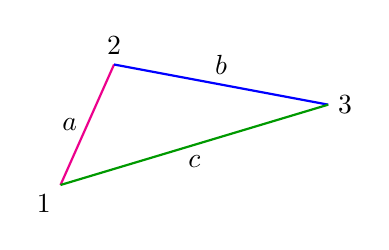
\begin{tikzpicture}[scale=.85]
\coordinate (v1) at (0,0);\coordinate (v2) at (.8,1.8);\coordinate (v3) at (4,1.2);
\draw[magenta,thick] (v1)--(v2) node[midway,left,text=black] {$a$};
\draw[blue,thick] (v2)--(v3) node[midway,above,text=black] {$b$};
\draw[green!60!black,thick] (v1)--(v3) node[midway,below,text=black] {$c$};
\node[below left] at (v1) {$1$};\node[above] at (v2) {$2$};\node[right] at (v3) {$3$};
\end{tikzpicture}
\caption{为记录标号, 我们给各条边着色.}\label{src:1.2.5}
\end{figure}
定义带标号三角形的模集合 $M$: 对象是带标号的三角形, 两个三角形等价, 是指它们是 $\mathbb R^2$ 中同一个三角形, 具有相同的顶点和相同的标号. 将带标号顶点的坐标记作 $(x_1,y_1)$, $(x_2,y_2)$ 和 $(x_3,y_3)$, 得到双射
\begin{equation}\label{src:1.2.6}
\begin{aligned}
M&\cong\left\{(x_1,y_1,x_2,y_2,x_3,y_3)\;\middle|\;
\det\begin{pmatrix}x_2-x_1&x_3-x_1\\y_2-y_1&y_3-y_1\end{pmatrix}\neq0\right\}\\
&\hspace{2em}\subseteq\mathbb R^6.
\end{aligned}
\end{equation}
即 $M$ 与 $\mathbb R^6$ 的一个开子集双射, 其补集是余维 $1$ 的闭子集, 由向量 $(x_2,y_2)-(x_1,y_1)$ 与 $(x_3,y_3)-(x_1,y_1)$ 线性相关这一条件定义.

\begin{figure}[htbp]
\centering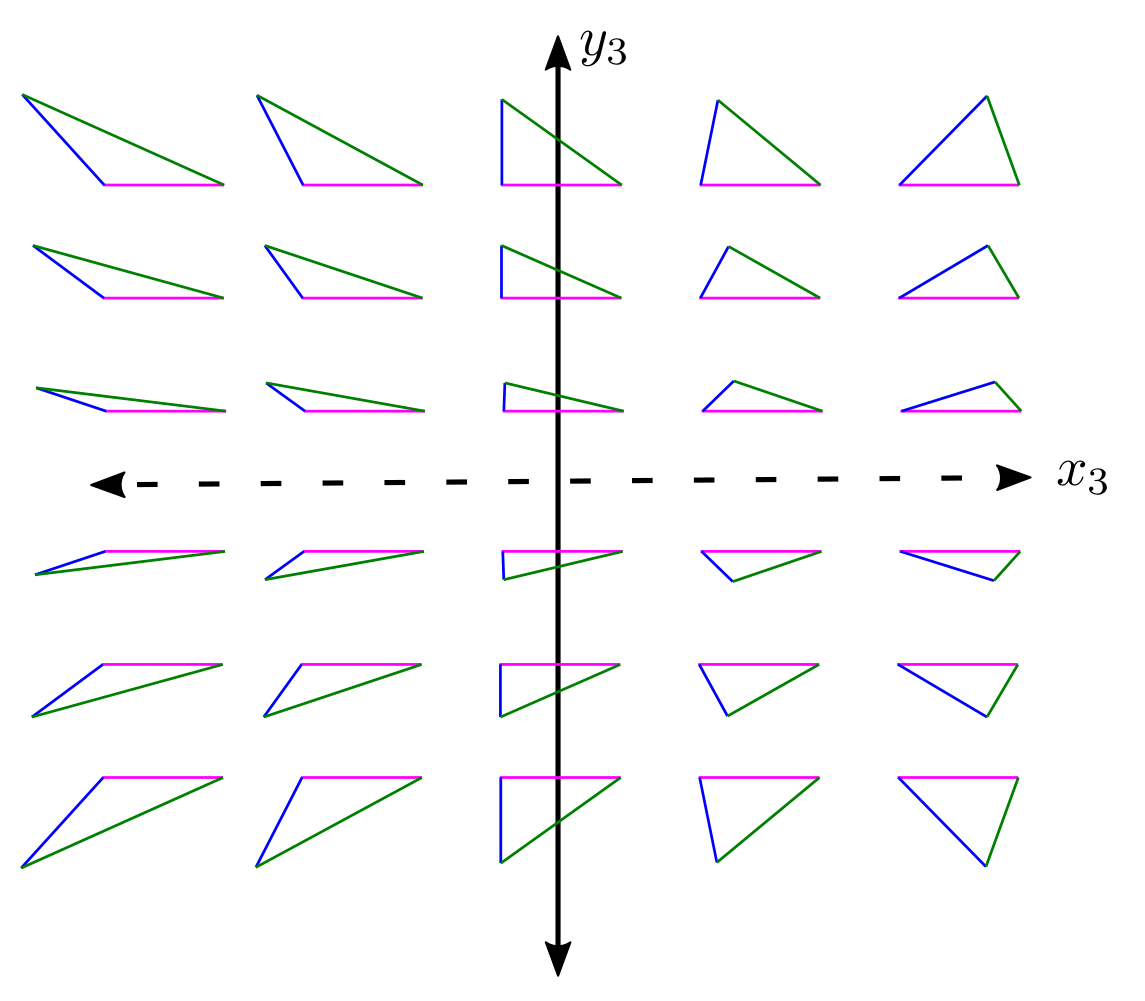
\includegraphics[width=.48\textwidth]{figures/fig-1.2.7.png}
\caption{模空间 $M$ 中 $(x_1,y_1)=(0,0)$, $(x_2,y_2)=(1,0)$ 的截面. 三角形由满足 $y_3\neq0$ 的第三个顶点 $(x_3,y_3)$ 描述. 我们为 $x_3y_3$ 平面中的一些点画出了代表三角形.}\label{src:1.2.7}
\end{figure}

\begin{example}[相似意义下带标号的三角形]\label{src:1.2.8}
定义相似意义下带标号三角形的模集合, 记作 $M^{\mathrm{lab}}$: 对象与前一个例子相同, 仍为带标号的三角形, 但等价关系改为保持标号的相似关系.
\end{example}
\begin{figure}[htbp]
\centering
\begin{tikzpicture}[scale=.7]
\draw[magenta,thick] (0,0)--(.8,1.8);
\draw[blue,thick] (.8,1.8)--(4,1.2);
\draw[green!60!black,thick] (4,1.2)--(0,0);
\node at (5.2,1.2) {$\sim$};\node at (5.2,.65) {相似};
\begin{scope}[shift={(8.7,0)},rotate=105]
\draw[magenta,thick] (0,0)--(.8,1.8);
\draw[blue,thick] (.8,1.8)--(4,1.2);
\draw[green!60!black,thick] (4,1.2)--(0,0);
\end{scope}
\node at (10.2,1.2) {$\not\sim$};\node at (10.2,.65) {不相似};
\draw[magenta,thick] (12,0)--(11.5,2.7);
\draw[blue,thick] (12,0)--(13.5,0);
\draw[green!60!black,thick] (11.5,2.7)--(13.5,0);
\end{tikzpicture}
\caption{左边的两个三角形相似, 但第三个与它们不相似.}\label{src:1.2.9}
\end{figure}
每个带标号的三角形都相似于唯一一个周长 $a+b+c=2$ 的带标号三角形. 得到描述
\begin{equation}\label{src:1.2.10}
M^{\mathrm{lab}}=\left\{(a,b,c)\;\middle|\;
\begin{aligned}
&a+b+c=2\\
&0<a<b+c\\
&0<b<a+c\\
&0<c<a+b
\end{aligned}\right\}.
\end{equation}
令 $c=2-a-b$, 便可以将 $M^{\mathrm{lab}}$ 直观呈现为 $\mathbb R^2$ 中由满足 $0<a,b<1$ 和 $a+b>1$ 的数对 $(a,b)$ 定义的解析开子集.

\begin{figure}[htbp]
\centering\begin{tikzpicture}[scale=5]
\fill[gray!25] (0,1)--(1,0)--(1,1)--cycle;
\draw[->] (0,0)--(1.12,0) node[right] {$a$};
\draw[->] (0,0)--(0,1.12) node[above] {$b$};
\draw[densely dotted] (0,1)--(1,0)--(1,1)--cycle;
\node[left] at (0,1) {$1$};\node[below] at (1,0) {$1$};
\draw[blue] (.5,.5)--(1,1);
\draw[blue] (0,1)--(1,.5);
\draw[blue] (.5,1)--(1,0);
\draw[magenta,thick,domain=0:1,samples=100] plot (\x,{(\x*\x-2*\x+2)/(2-\x)});
\draw[magenta,thick,domain=0:1,samples=100] plot ({(\x*\x-2*\x+2)/(2-\x)},\x);
\draw[magenta,thick,domain=0:1,samples=100] plot (\x,{(2-2*\x)/(2-\x)});
\fill[green!75!black] (2/3,2/3) circle (.012);
\node[font=\small,rotate=-45,fill=white,inner sep=1pt] at (.38,.55) {退化三角形};
\draw[->,gray] (1.3,.7)--(.87,.87);\node[right,font=\small] at (1.25,.73) {等腰三角形};
\draw[->,gray] (1.2,.53)--(.69,.66);\node[right,font=\small] at (1.15,.5) {等边三角形};
\draw[->,gray] (.43,.1)--(.7,{(2-2*.7)/(2-.7)});\node[below,font=\small] at (.4,.1) {直角三角形};
\end{tikzpicture}

\caption{$M^{\mathrm{lab}}$ 是阴影三角形. 品红色曲线表示由 $a^2+b^2=c^2$, $a^2+c^2=b^2$ 和 $b^2+c^2=a^2$ 定义的直角三角形, 蓝色直线表示由 $a=b$, $b=c$ 和 $a=c$ 定义的等腰三角形, 绿色点是由 $a=b=c$ 定义的唯一的等边三角形.}\label{src:1.2.11}
\end{figure}

\begin{example}[相似意义下无标号的三角形]\label{src:1.2.12}
现在转向相似意义下无标号三角形的模, 它呈现出前两个例子中未见的新特征: 对称性!
\end{example}
定义相似意义下无标号三角形的模集合, 记作 $M^{\mathrm{unl}}$: 对象是 $\mathbb R^2$ 中无标号的三角形, 等价关系为相似关系. 通过按递增次序排列边长的有序三元组 $(a,b,c)$, 可以唯一描述一个无标号三角形: 
\begin{equation}\label{src:1.2.13}
M^{\mathrm{unl}}=\left\{(a,b,c)\;\middle|\;
\begin{aligned}
&0<a\leq b\leq c<a+b\\
&a+b+c=2
\end{aligned}\right\}.
\end{equation}
\begin{figure}[H]
\centering\begin{tikzpicture}[scale=5.5]
\fill[gray!30] (0,1)--(.5,.5)--(2/3,2/3)--cycle;
\draw[->] (0,0)--(1.08,0) node[right] {$a$};
\draw[->] (0,0)--(0,1.1) node[above] {$b$};
\draw[densely dotted] (0,1)--(.5,.5);
\draw[blue] (0,1)--(2/3,2/3)--(.5,.5);
\draw[magenta,thick,domain=0:{2-sqrt(2)},samples=100] plot (\x,{(2-2*\x)/(2-\x)});
\fill[green!75!black] (2/3,2/3) circle (.012);
\foreach \v/\t in {0.5/{1/2},0.6666667/{2/3}} {
\draw (\v,0)--(\v,-.02) node[below] {$\t$};
\draw (0,\v)--(-.02,\v) node[left] {$\t$};
}
\node[left] at (0,1) {$1$};
\node[font=\small,rotate=-45,fill=white,inner sep=1pt] at (.2,.75) {退化 $a+b=c$};
\node[font=\small,rotate=-27,above] at (.25,.9) {等腰 $b=c$};
\node[font=\small,rotate=45,below] at (.59,.57) {等腰 $a=b$};
\draw[->,gray] (.93,.86)--(.68,.68);\node[right,font=\small] at (.8,.89) {等边};
\draw[->] (.16,.25)--(.43,{(2-2*.43)/(2-.43)});
\node[font=\small,align=center] at (.17,.18) {直角三角形\\$a^2+b^2=c^2$};
\end{tikzpicture}

\caption{$M^{\mathrm{unl}}$ 的图像.}\label{src:1.2.14}
\end{figure}
满足 $a=b$ 或 $b=c$ 的等腰三角形, 以及满足 $a=b=c$ 的等边三角形, 其对称群分别为 $\mathbb Z/2$ 和 $S_3$. 遗憾的是, 上述 $M^{\mathrm{unl}}$ 的描述并未编码这一信息. 注意, 在 $S_3$ 对标号的自然作用下, 可以把 $M^{\mathrm{unl}}$ 等同于商 $M^{\mathrm{lab}}/S_3$; 而等腰三角形和等边三角形的稳定子, 恰好就是其对称群 $\mathbb Z/2$ 和 $S_3$. 在既非等腰又非等边的三角形轨迹上, $S_3$ 的作用是自由的.
